\begin{figure}
\centering
% \hspace{-.08\linewidth}
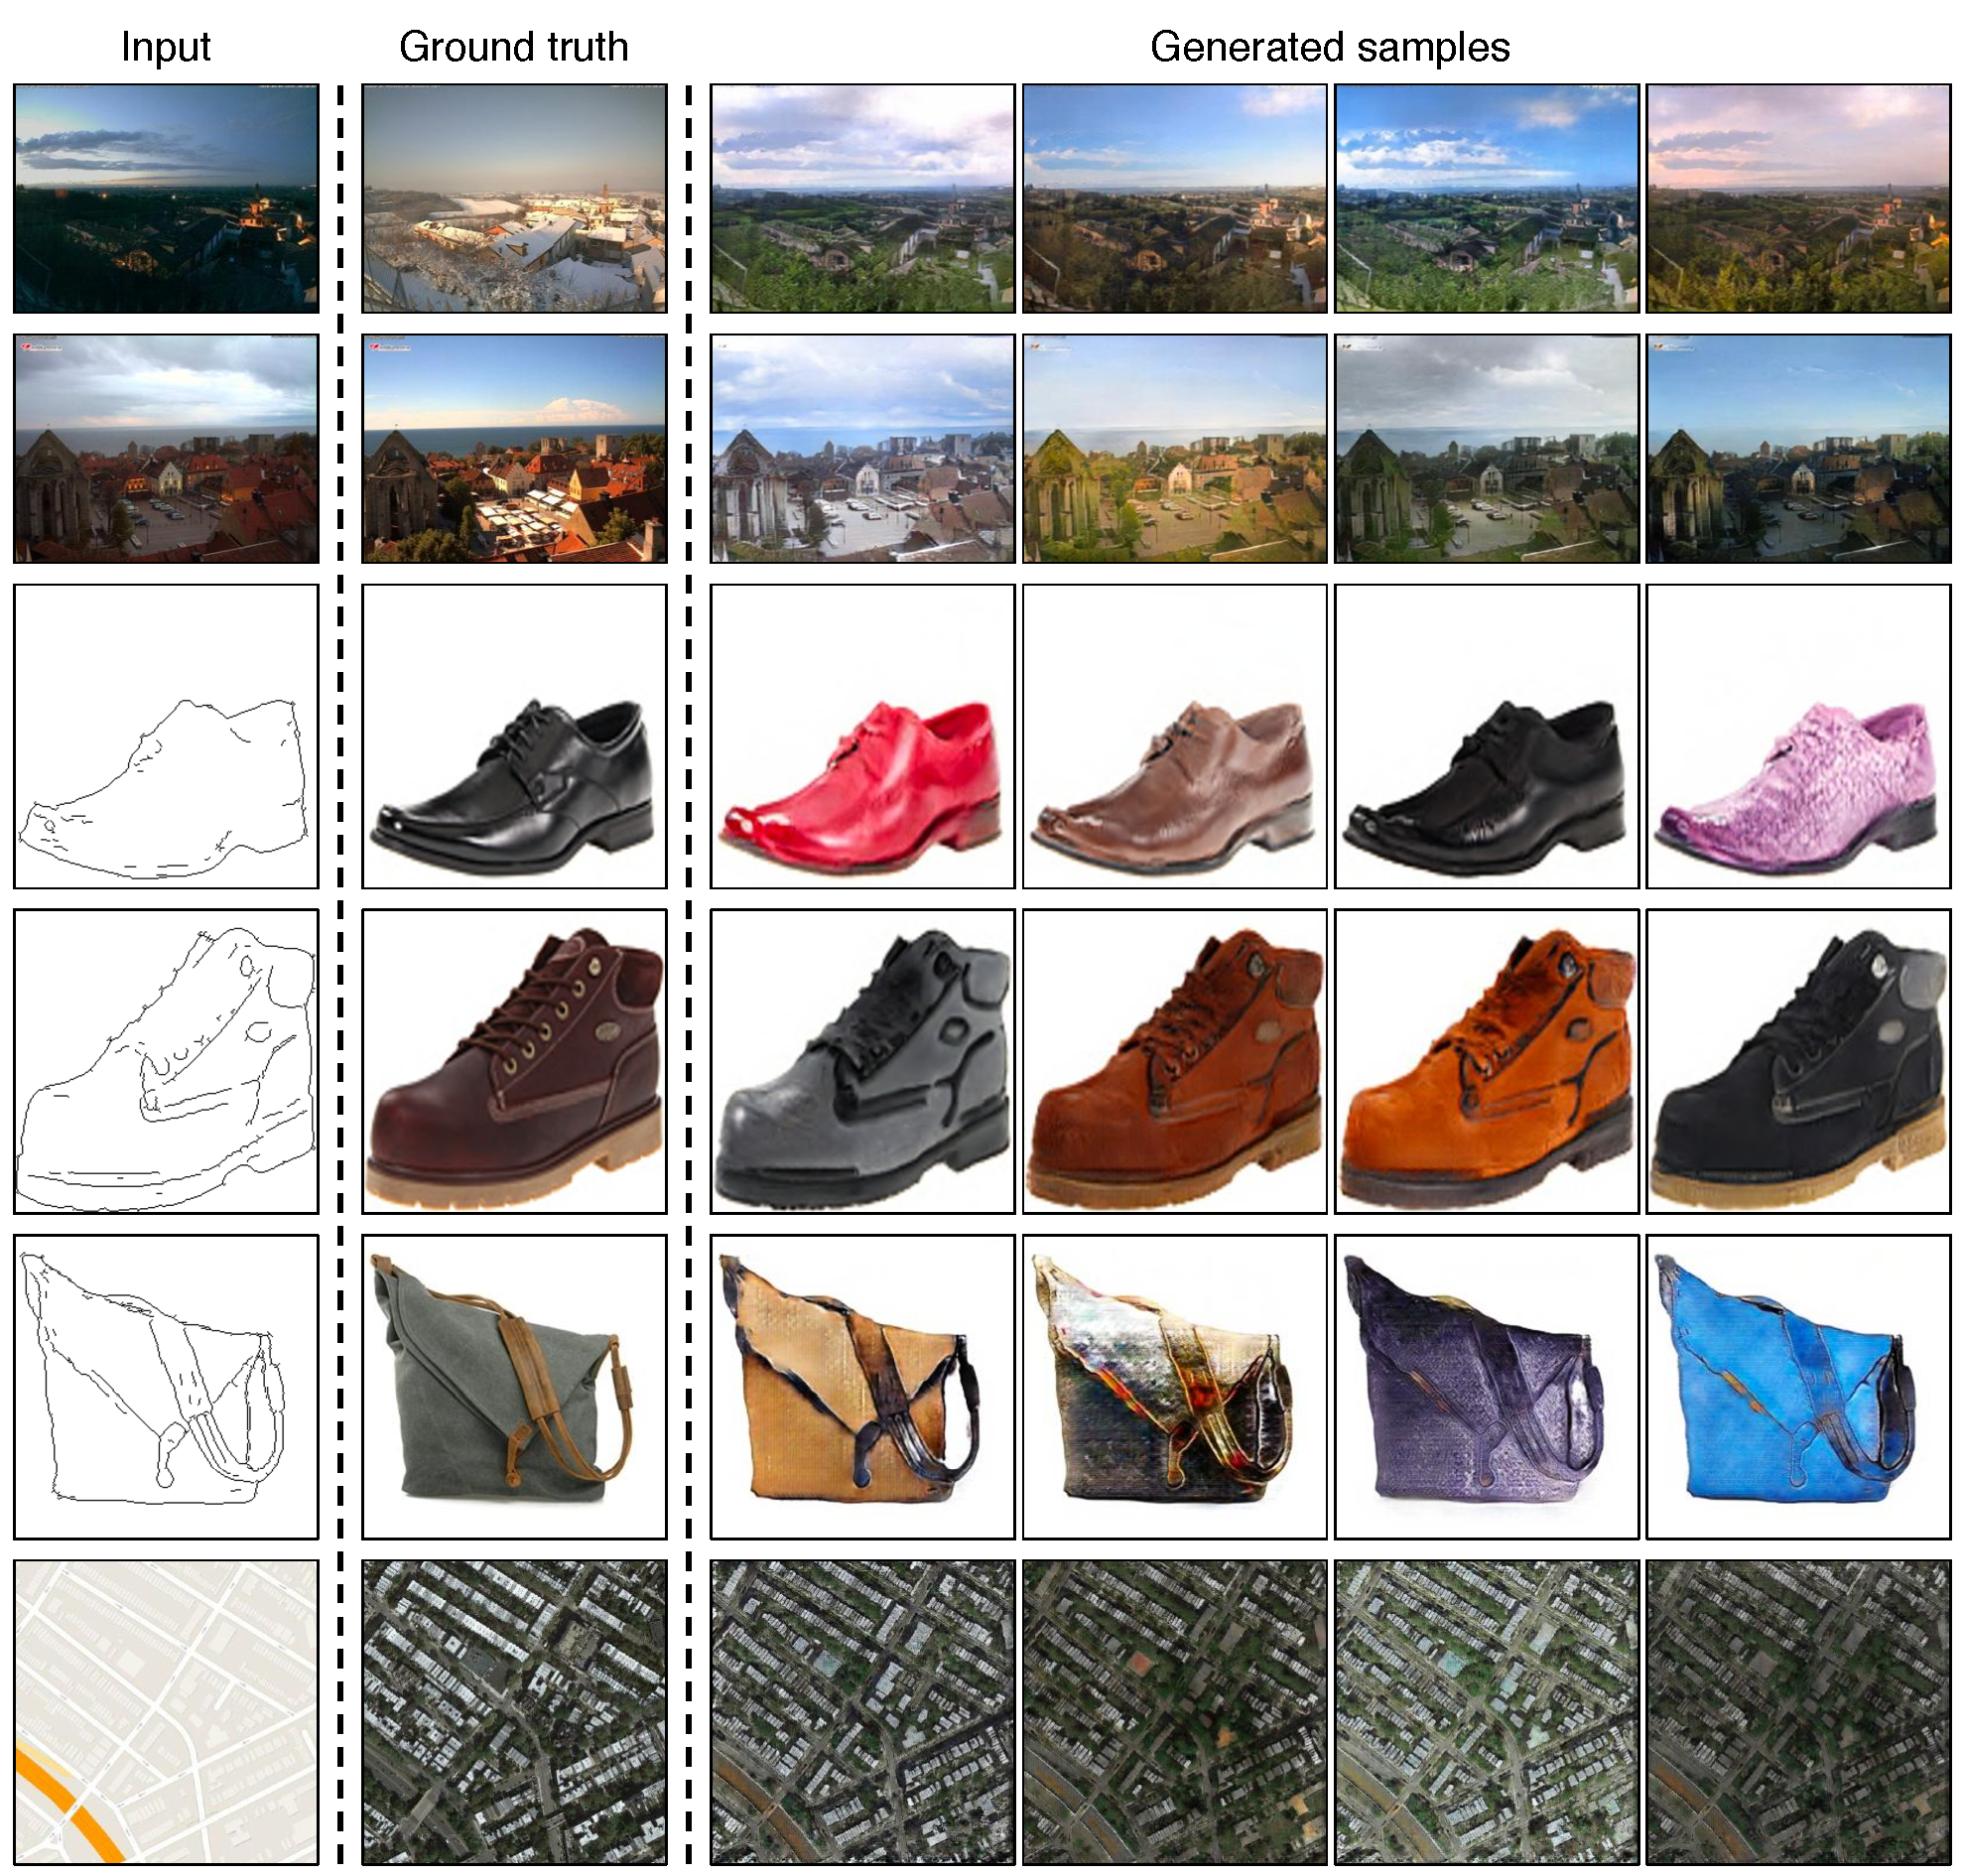
\includegraphics[width=1.\linewidth]{imgs/results_matrix.pdf}
\caption{\small \textbf{Example Results} We show example results of our hybrid model \bicycle. The left column shows the input. The second shows the ground truth output. The final four columns show randomly generated samples. We show results of our method on night$\rightarrow$day, edges$\rightarrow$shoes, edges$\rightarrow$handbags, and maps$\rightarrow$satellites. Models and additional examples are available at \url{https://junyanz.github.io/BicycleGAN}.} 
\vspace{-2mm}
\label{fig:results}
\end{figure}

\begin{figure}
\centering
\hspace{\linewidth}
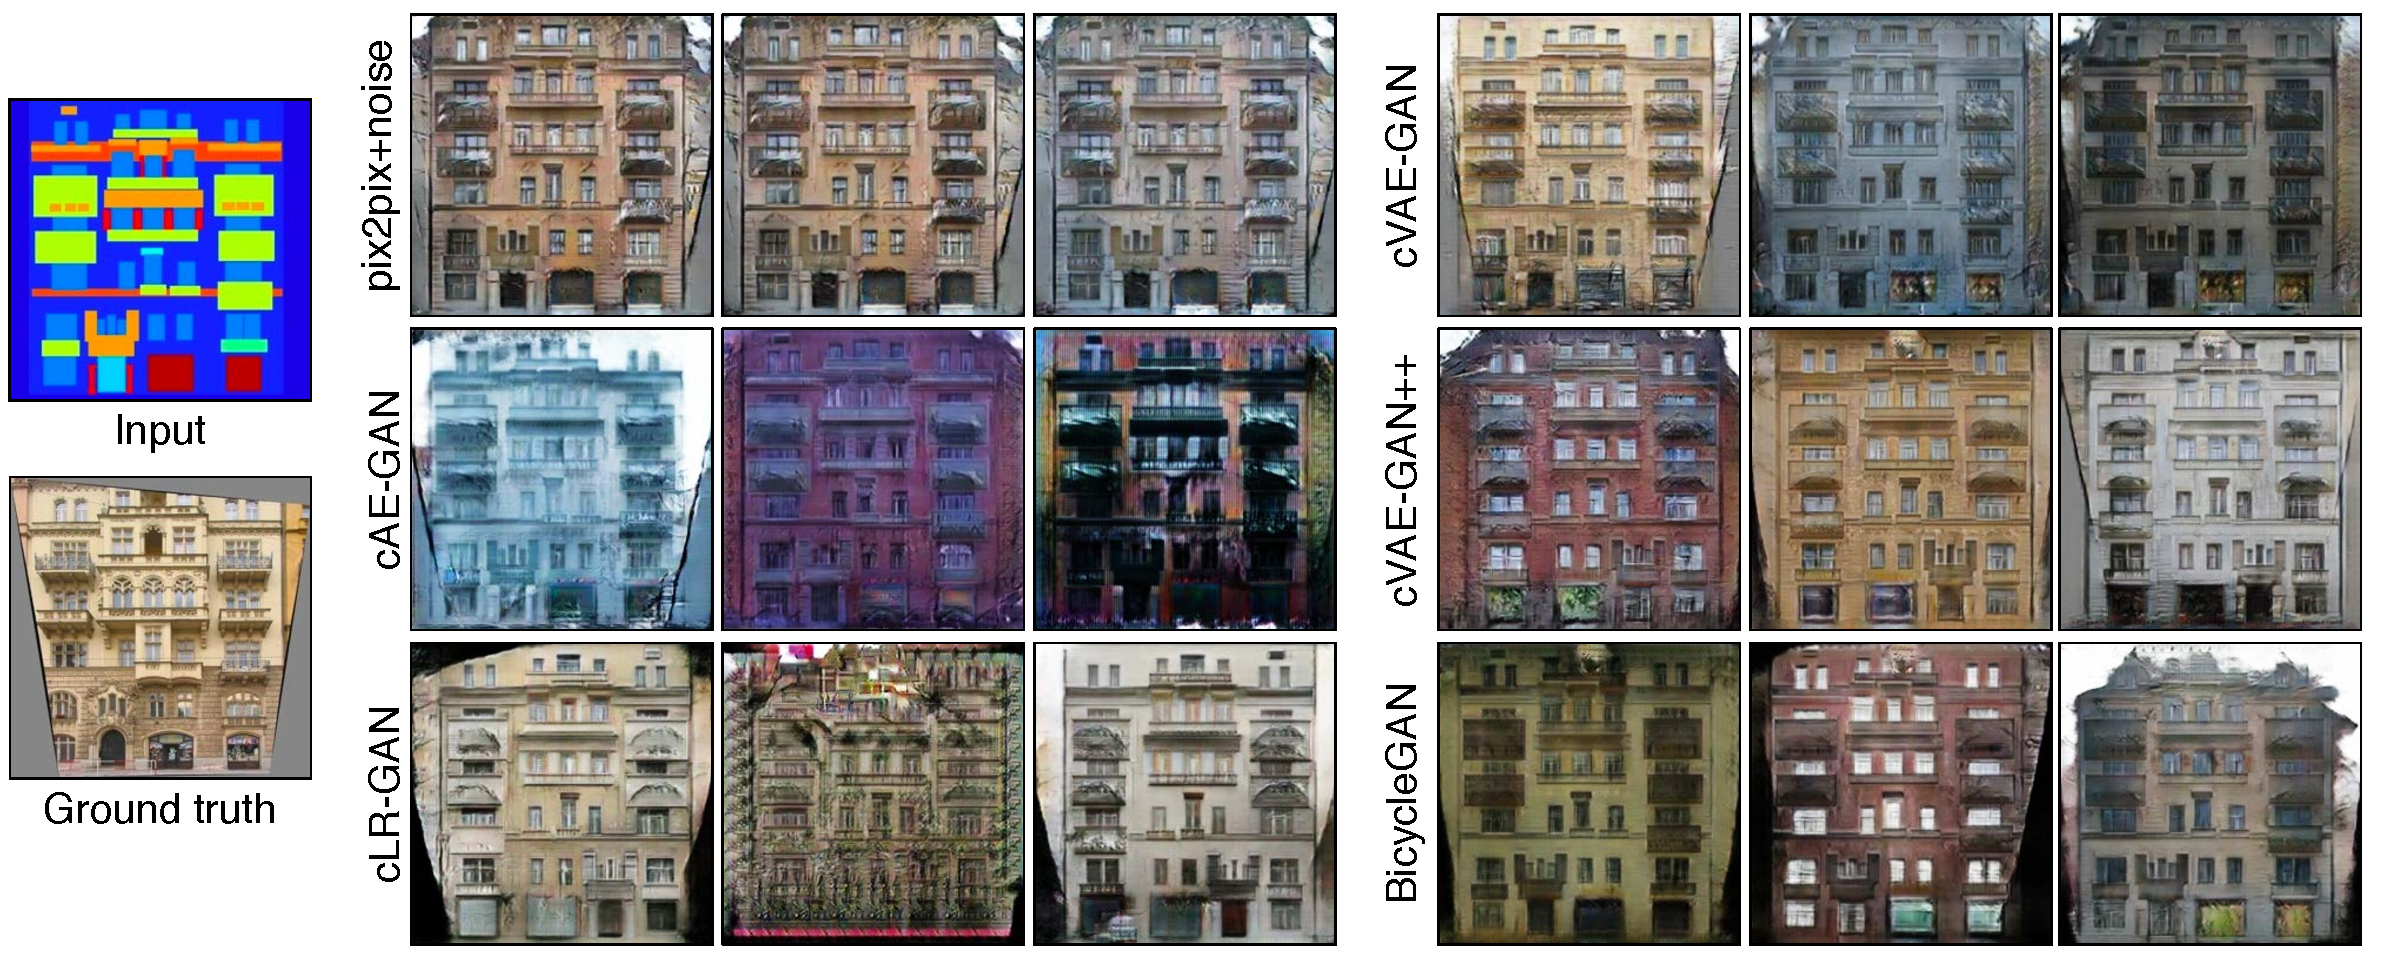
\includegraphics[width=\linewidth]{imgs/facades_comparison.pdf}
\caption{\small \textbf{Qualitative method comparison} We compare results on the labels $\rightarrow$ facades dataset across different methods. The \bicycle method produces results which are both realistic and diverse.}
\label{fig:resultsFacades}
\end{figure}

\section{Experiments}
\label{sec:exp}
\begin{figure}
  \centering
  \begin{minipage}[b]{0.54\linewidth}  
  \scalebox{0.92} {
  \begin{tabular}{l c c}
	& \textbf{Realism} & \textbf{Diversity} \\ \hline
	& AMT Fooling & LPIPS \\
	\textbf{Method} & Rate [\%] & Distance \\ \hline
	Random real images & 50.0\% & .262$\pm$.007 \\ \hline
	\ppn~\citep{isola2016image} & 27.93$\pm$2.40 \% & .013$\pm$.000 \\
	\cae & 13.64$\pm$1.80 \% & .204$\pm$.002 \\
	\cvaegan & 24.93$\pm$2.27 \% & .096$\pm$.001 \\
	\cvaeganp & 29.19$\pm$2.43 \% & .098$\pm$.002 \\
	\cinfogan & 29.23$\pm$2.48 \% & \footnote{We found that \cinfogan resulted in severe mode collapse, resulting in $\sim15\%$ of the images producing the same result. Those images were omitted from this calculation.}.090$\pm$.002 \\
	\bicycle & 34.33$\pm$2.69 \% & .110$\pm$.002 \\ \hline
	\end{tabular} } \\
	
  \end{minipage}
  \begin{minipage}[b]{0.45\linewidth}
  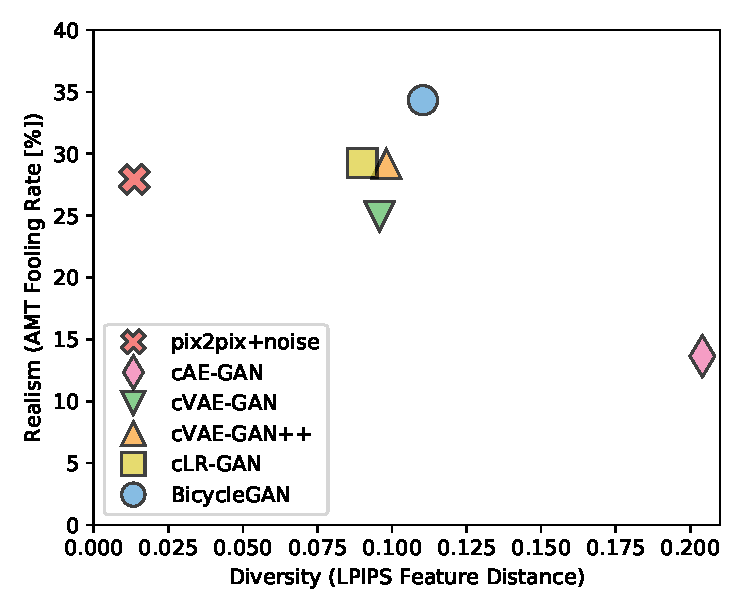
\includegraphics[width=\linewidth]{imgs/real_div.pdf} 
  \end{minipage}
  \vspace{-4mm}
  \caption{\small \textbf{Realism vs Diversity}. We measure diversity using average LPIPS distance~\cite{zhang2018unreasonable}, and realism using a real vs. fake Amazon Mechanical Turk test on the Google maps $\rightarrow$ satellites task. The \ppn baseline produces little diversity. Using only \cae method produces large artifacts during sampling. The hybrid \bicycle method, which combines \cvaegan and \cinfogan, produces results which have higher realism while maintaining diversity.
  }
  \vspace{-5mm}
  \label{fig:real_vs_div}
\end{figure}


{\bf Datasets} We test our method on several image-to-image translation problems from prior work, including edges $\rightarrow$ photos~\citep{yu2014fine,zhu2016generative}, Google maps $\rightarrow$ satellite~\citep{isola2016image}, labels $\rightarrow$ images~\citep{Cordts2016Cityscapes}, and outdoor night $\rightarrow$ day images~\citep{Laffont14}. These problems are all one-to-many mappings. We train all the models on $256\times 256$ images.


{\bf Methods} We evaluate the following models described in Section \ref{sec:methods}: \ppn, \cae, \cvaegan, \cvaeganp, \cinfogan, and our hybrid model \bicycle.

\subsection{Qualitative Evaluation}
\vspace{-1mm}
We show qualitative comparison results on Figure \ref{fig:resultsFacades}. We observe that \ppn typically produces a single realistic output, but does not produce any meaningful variation.
\cae adds variation to the output, but typically at a large cost to result quality. An example on facades is shown on Figure~\ref{fig:results}.

We observe more variation in the \cvaegan, as the latent space is encouraged to encode information about ground truth outputs. However, the space is not densely populated, so drawing random samples may cause artifacts in the output. The \cinfogan shows less variation in the output, and sometimes suffers from mode collapse. When combining these methods, however, in the hybrid method \bicycle, we observe results which are both diverse and realistic. Please see our website for a full set of results.

\vspace{-1mm}
\subsection{Quantitative Evaluation}
\vspace{-1mm}
We perform a quantitative analysis of the diversity, realism, and latent space distribution on our six variants and baselines. We quantitatively test the Google maps $\rightarrow$ satellites dataset.

% {\bf Does the system produce \textit{diverse} results?}
{\bf Diversity} We compute the average distance of random samples in deep feature space. Pretrained networks have been used as a ``perceptual loss" in image generation applications~\citep{gatys2016image,johnson2016perceptual,dosovitskiy2016generating}, as well as a held-out ``validation" score in generative modeling, for example, assessing the semantic quality and diversity of a generative model~\citep{salimans2016improved} or the semantic accuracy of a grayscale colorization~\citep{zhang2016colorful}.

In Figure~\ref{fig:real_vs_div}, we show the diversity-score using the LPIPS metric proposed by~\cite{zhang2018unreasonable}\footnote{Learned Perceptual Image Patch Similarity (LPIPS) metric computes distance in AlexNet~\cite{krizhevsky2014one} feature space (\texttt{conv1-5}, pretrained on Imagenet~\citep{russakovsky2015imagenet}), with linear weights to better match human perceptual judgments.}. For each method, we compute the average distance between 1900 pairs of randomly generated output $\Bh$ images (sampled from 100 input $\A$ images). Random pairs of ground truth real images in the $\B \in \mathcal{B}$ domain produce an average variation of .262. As we are measuring samples $\Bh$ which correspond to a specific input $\mathbf{A}$, a system which stays faithful to the input should definitely not exceed this score.

The \pp system~\citep{isola2016image} produces a single point estimate. Adding noise to the system \ppn produces a small diversity score, confirming the finding in~\citep{isola2016image} that adding noise does not produce large variation. Using the \cae model to encode a ground truth image $\B$ into a latent code $\z$ does increase the variation. The \cvaegan, \cvaeganp, and \bicycle models all place explicit constraints on the latent space, and the \cinfogan model places an implicit constraint through sampling. These four methods all produce similar diversity scores. We note that high diversity scores may also indicate that unnatural images are being generated, causing meaningless variations. Next, we investigate the visual realism of our samples.

{\bf Perceptual Realism} To judge the visual realism of our results, we use human judgments, as proposed in~\citep{zhang2016colorful} and later used in~\citep{isola2016image,zhu2017unpaired}. The test sequentially presents a real and generated image to a human for 1 second each, in a random order, asks them to identify the fake, and measures the ``fooling" rate. %An algorithm which produces perfectly realistic images would achieve a score of 50\% by definition, and higher is better. 
Figure \ref{fig:real_vs_div}(left) shows the realism across methods. The \ppn model achieves high realism score, but without large diversity, as discussed in the previous section. 
The \cae helps produce diversity, but this comes at a large cost to the visual realism. Because the distribution of the learned latent space is unclear, random samples may be from unpopulated regions of the space. Adding the KL-divergence loss in the latent space, used in the \cvaegan model, recovers the visual realism. Furthermore, as expected, checking randomly drawn $\z$ vectors in the \cvaeganp model slightly increases realism. The \cinfogan, which draws $\z$ vectors from the predefined distribution randomly, produces similar realism and diversity scores. However, the \cinfogan model resulted in large mode collapse - approximately $15\%$ of the outputs produced the same result, independent of the input image. The full hybrid \bicycle gets the best of both worlds, as it does not suffer from mode collapse and also has the highest realism score by a significant margin.  

\begin{table}
\begin{center}
 \begin{tabular}{l c c c c}
	Encoder & \texttt{E\textsubscript{ResNet}}  &  \texttt{E\textsubscript{ResNet}} &  \texttt{E\textsubscript{CNN}}  &  \texttt{E\textsubscript{CNN}} \\ \hline
	Injecting $\z$ & \texttt{add\_to\_all} &  \texttt{add\_to\_input} & \texttt{add\_to\_all} &  \texttt{add\_to\_input}\\ \hline
	label$\rightarrow$photo & $0.292 \pm 0.058$ & $0.292 \pm0.054$ & $0.326\pm 0.066$& $0.339\pm 0.069$ \\
	map $\rightarrow$ satellite &  $0.268 \pm 0.070$  & $0.266 \pm 0.068$ & $0.287 \pm 0.067$&$0.272\pm 0.069$\\
    \hline
	\end{tabular}
		\caption{The encoding performance with respect to the different encoder architectures and methods of injecting $\z$. Here we report the reconstruction loss $||\B - \G(\A,\E(B)) ||_1$}.
			\label{tab:rec}
	\end{center}
\vspace{-10mm}
\end{table}

{\bf Encoder architecture} In \pp, ~\citet{isola2016image} conduct extensive ablation studies on discriminators and generators. Here we focus on the performance of two encoder architectures, \texttt{E\textsubscript{CNN}} and \texttt{E\textsubscript{ResNet}}, for our applications on the maps and facades datasets. We find that \texttt{E\textsubscript{ResNet}} better encodes the output image, regarding the image reconstruction loss $||\B - \G(\A,\E(B)) ||_1$ on validation datasets as shown in Table~\ref{tab:rec}. We use \texttt{E\textsubscript{ResNet}} in our final model.

{\bf Methods of injecting latent code} We evaluate two ways of injecting latent code $\z$: \texttt{add\_to\_input} and \texttt{add\_to\_all} (Section ~\ref{sec:implementation}), regarding the same reconstruction loss $||\B - \G(\A,\E(B)) ||_1$. Table~\ref{tab:rec} shows that two methods give similar performance. This indicates that the \texttt{U\_Net}~\cite{ronneberger2015u} can already propagate the information well to the output without the additional skip connections from $\z$. We use \texttt{add\_to\_all} method to inject noise in our final model.

\begin{figure}
  \centering
  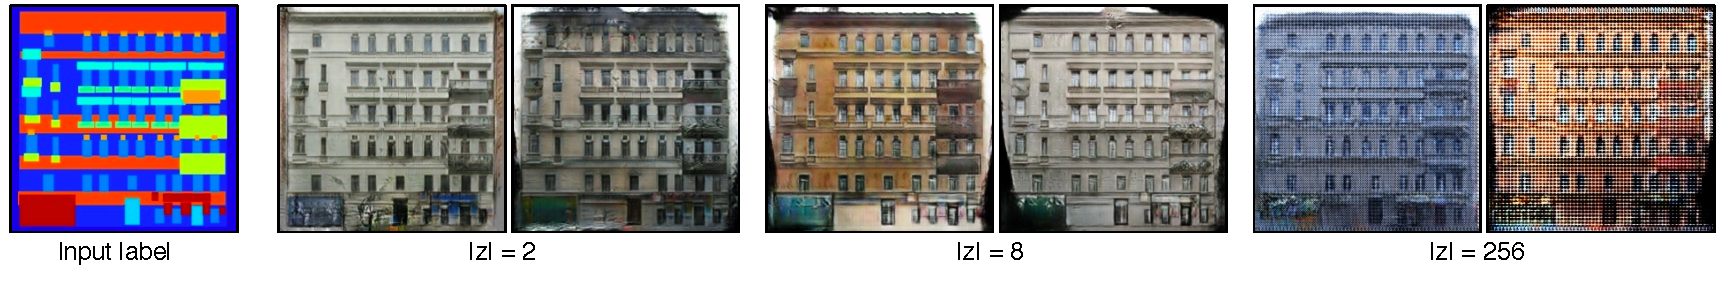
\includegraphics[width=1.\linewidth]{imgs/nz_facades.pdf}
\vspace{-4mm}
\caption{Different label $\rightarrow$ facades results trained with varying length of the latent code $|\z| \in \{2, 8, 256\}$. }
\label{fig:numberofz}
\vspace{-6mm}
\end{figure}


{\bf Latent code length} We study the \bicycle model results with respect to the varying number of dimensions of latent codes $\{2, 8, 256\}$ in Figure~\ref{fig:numberofz}. A very low-dimensional latent code may limit the amount of diversity that can be expressed. On the contrary, a very high-dimensional latent code can potentially encode more information about an output image, at the cost of making sampling difficult. The optimal length of $\z$ largely depends on individual datasets and applications, and how much ambiguity there is in the output. 

\vspace{-2mm}